\chapter{Radio Networks}

Una \textbf{radio network} è un insieme di \textit{dispositivi} fisici collocati in uno \textbf{spazio euclideo}, ognuno dei quali dotato di un trasmettitore \textit{radio (wireless)}. Ogni nodo $v$ della rete ha un fissato \textbf{raggio di trasmissione} $r(v) > 0$, entro il quale potrà trasmettere il suo segnale. Un qualsiasi nodo $w$ per ricevere un messaggio $v$ deve essere ad una \textit{distanza} minore del raggio di trasmissione $r(v)$
\[
    d(v, w) = \norm{v - w} \leq r(v)
\]

Inoltre il nodo $v$ non può selezionare a quale dei suoi nodi vicini inviare il messaggio e a quali no: il messaggio verrà trasmesso in \textit{broadcast} a tutti i nodi entro il raggio di trasmissione di $v$. Questo tipo di comunicazione è detta \textbf{node based}.

Data quindi una rete radio, si può costruire un \textbf{grafo diretto delle comunicazione}, in cui esiste l'arco $(u, v)$ solo se $v$ è coperto dal raggio di trasmissione di $u$.

Le reti radio sono anche dette \textbf{unknown} in quanto i nodi non hanno nessuna conoscenza in merito agli altri nodi e alla loro posizione, perciò è come considerare un grafo in cui i nodi non conoscono il loro vicinato, in cui hanno una sola porta dalla quale trasmettere il messaggio e basta.

Infine le reti radio sono considerate essere un sistema completamente \textbf{sincrono}. Tutti i nodi condividono un \textbf{clock globale}, perciò diremo che i nodi agiscono in \textbf{time slots}. Inoltre si assume che i messaggi vengono trasmessi nella propria area di trasmissione in un unico time slot.

\textbf{Modello d'interferenza} \\
In un contesto reale, in genere, se troppi dispositivi trasmettono nello stesso momento e in una stessa area si crea troppo \textit{rumore/interferenza}. In una rete radio quindi, se un nodo $v$ riceve più di un messaggio in uno stesso time slot, assumeremo che si crei un'interferenza e che quindi $v$ non ha ricevuto il messaggio.

Più formalmente diremo che il nodo $v$ viene informato al time slot $t > 0$ se e solo se esiste un \textbf{unico} suo vicino che gli trasmette il messaggio al tempo $t$.

\begin{figure}[htbp]
    \centering
    
    % --- PRIMA SOTTOFIGURA ---
    \begin{subfigure}[b]{0.5\textwidth}
        \centering
        \resizebox{\linewidth}{!}{% Adatta l'immagine alla larghezza della sottofigura
            \begin{tikzpicture}
                % Stile per i nodi (punti centrali)
                \tikzset{
                    node point/.style={
                        circle,
                        fill=nodeblue,
                        inner sep=0pt,
                        minimum size=4.5mm
                    }
                }
            
                % Nodi e coperture
                \draw (-1.0, 1.7) circle (2.2);
                \node[node point] at (-1.0, 1.7) {};
            
                \draw (-2.6, 0.3) circle (1.5);
                \node[node point] at (-2.6, 0.3) {};
            
                \draw (-1.4, 0.0) circle (1.1);
                \node[node point] at (-1.4, 0.0) {};
            
                \draw (-0.6, 0.0) circle (1.1);
                \node[node point] at (-0.6, 0.0) {};
            
                \draw (1.6, -0.2) circle (2.5);
                \node[node point] at (1.6, -0.2) {};
            
                \draw (-1.8, -1.6) circle (2.3);
                \node[node point] at (-1.8, -1.6) {};
            
                \draw (-0.1, -1.8) circle (2.1);
                \node[node point] at (-0.1, -1.8) {};
            \end{tikzpicture}
        }
        \caption{Raggi di copertura}
        \label{fig:copertura}
    \end{subfigure}
    \hfill % Aggiunge spazio flessibile tra le due sottofigure
    % --- SECONDA SOTTOFIGURA ---
    \begin{subfigure}[b]{0.45\textwidth}
        \centering
        \resizebox{\linewidth}{!}{% Adatta l'immagine alla larghezza della sottofigura
            \begin{tikzpicture}[>=Stealth, thick, node distance=1.5cm, every node/.style={circle, fill=graphcyan, minimum size=8mm, draw=black!30}]
            
              % Coordinate dei nodi
              \node (top) at (0, 3.5) {};
              \node (left) at (-3, 1.8) {};
              \node (midleft) at (-1.2, 1.5) {};
              \node (midright) at (0.6, 1.5) {};
              \node (right) at (3.8, 1.0) {};
              \node (botleft) at (-1.8, -1.0) {};
              \node (botright) at (1.8, -1.8) {};
            
              % Archi dal nodo superiore
              \draw[->] (top) -- (left);
              \draw[->] (top) -- (midleft);
              \draw[->] (top) -- (midright);
            
              % Archi dal nodo a sinistra
              \draw[->] (left) -- (midleft);
            
              % Collegamento bidirezionale centrale
              \draw[<->] (midleft) -- (midright);
            
              % Archi dal nodo a destra
              \draw[->] (right) -- (midright);
              \draw[->] (right) -- (botright);
            
              % Archi e collegamenti inferiori
              \draw[->] (botright) -- (midright);
              \draw[<->] (botright) -- (botleft);
            
              % Archi dal nodo inferiore-sinistro
              \draw[->] (botleft) -- (left);
              \draw[->] (botleft) -- (midleft);
              \draw[->] (botleft) -- (midright);
            
            \end{tikzpicture}
        }
        \caption{Topologia del grafo diretto}
        \label{fig:grafo}
    \end{subfigure}
    
    \caption{Rappresentazione della rete: (a) schema delle aree di copertura dei nodi e (b) i relativi collegamenti.}
    \label{fig:rete_completa}
\end{figure}

\newpage
\section{Broadcast on Radio Networks}

Uno dei \textit{task} più comuni in un ambiente reale è quello del broadcast di un segnale su una rete radio. Come accennato, questo task soffre del problema dell'interferenza, perciò si vuole trovare un protocollo che porti a termine il broadcast di un'informazione considerando questa ulteriore difficoltà.

Modelliamo quindi il problema considerando come grafo il \textbf{grafo di comunicazione} $G = (V, E)$, grafo diretto derivato dalla rete radio, dove $V$ è l'insieme dei nodi partecipanti alla rete. mentre 
\[
    E = \{ (u,v): u,v \in V \land \norm{u, v} \leq r(u) \}
\]
Valgono inoltre le seguenti assunzioni:
\begin{itemize}
    \item \textbf{Sistem sincrono:} ogni nodo condivide uno stesso \textit{clock globale} che scandisce le azioni.
    \item \textbf{Unica sorgente} $s$ che avvia il protocollo
    \item \textbf{Connettività} di $G$, deve essere \textit{fortemente connesso} in quanto la sorgente può essere scelta arbitrariamente dall'avversario.
    \item \textbf{Presenza di interferenze:} un nodo $v$ viene informato al tempo $t > 0$ se esiste un \textit{unico} nodo che al tempo $t-1$ gli trasmette il messaggio.
    \item \textbf{Total Reliability:} non si verificano faults (eccetto le interferenze)
\end{itemize}

Come primo protocollo potremmo considerare il \texttt{Flooding}. È facile trovare un controesempio in cui il protocollo non informerà mai tutti i nodi

\begin{figure}[h]
    \centering
    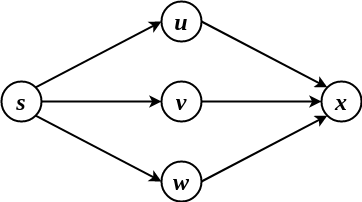
\includegraphics[width=0.6\textwidth]{images/radionet3.png}
    \caption{Controesempio in cui il protocollo \texttt{Flooding} non funziona.}
\end{figure}\label{fig:counterexampleflood}

Consideriamo il grafo nella \autoref{fig:counterexampleflood}, e supponiamo che la sorgente sia il nodo $s$. Al time slot $t_0$ la sorgente $s$ invierà il messaggio ai nodi $u,v,w$ e al time slot successivo i nodi $u,v,w$ invieranno il messaggio al nodo $x$, causando un interferenza. Dopo che $u,v,w$ avranno trasmesso, essi entreranno nello stato \texttt{done} e non trasmetteranno mai più. Così facendo il nodo $x$ non riceverà \textbf{mai} il messaggio, e il task non sarà mai risolto.

\subsection{Round-Robin Protocol}

Assumiamo che i nodi siano univocamente identificati da un valore nell'intervallo $[1,n]$, e ciascun nodo è a conoscenza della propria etichetta. Assumiamo inoltre che tutti i nodi conoscano una \textbf{buona approssimazione} di $n$. Per semplicità al momento assumiamo che conoscoano il valore esatto di $n$.

L'idea del protocollo \texttt{Round-Robin (RR)} è quella di scandire il protocollo in \textbf{fasi} con durata complessiva di $n$ time slots ciascuna. Dato che ogni fase $k \geq 0$ dura esattamente $n$ istanti, ogni nodo con etichetta $i$ trasmetterà al time slot $i-$esimo della fase $k$. Più formalmente, per ogni fase $k \geq 0$, il nodo $i$ può trasmettere solo negli istanti $kn + i$. Importante osservare che è possibile definire una scansione temporale delle azioni da svolgere grazie all'assunzione di sincronismo del sistema. Questo sistema ci garantisce che non è possibile che accada una situazione d'interferenza, in quanto può trasmetere un solo nodo alla volta.

\begin{algorithm}
\caption{Round-Robin Protocol}
\begin{algorithmic}[1]
\For{phase $j = 0, 1, 2, \dots$}
    \For{time $= jn, jn+1, \dots, (j+1)n-1$}
        \If{$id(x) \equiv \text{time} \pmod n\ \land$ state(x) = \texttt{informed}}
            \State \texttt{send(msg)}
            \State state(x) $\gets$ \texttt{done}
        \EndIf
    \EndFor
\EndFor
\end{algorithmic}
\end{algorithm}

\textbf{Osservazione:} Per come è definito il protocollo, questo non termina mai. Si mostrerà nell'analisi del protocollo che è sufficiente eseguire $n$ fasi.

\subsection{Analisi Round-Robin}

\begin{teorema}[Correttezza]
    Sotto le precedenti assunzioni, nel protocollo \texttt{RR}, tutti i nodi a distanza $k$ (distanza nel numero di archi, non euclidea) dalla sorgente $s$ verranno informati \textbf{entro} $k$ fasi.
    \begin{proof}
        Dimostriamo per induzione su $k$.
        \begin{description}
            \item[Passo Base] Nella prima fase, il primo nodo a trasmattere sarà la sorgente $s$ nel time slot $id(s)$; inoltre, in tale time-slot $s$ è l'unico nodo a trasmettere. Allora tutti i vicini di $s$ nel grafo delle comunicazioni, ossia i nodi a distanza 1 da $s$, per via del modello radio network, ricevono correttamente il messaggio.
            \item[Passo Induttivo] Supponiamo quindi per ipotesi induttiva che sia vero che per ogni fase $k > 0$ ogni nodo nell'insieme
            \[
                L_k := \{v \in V: d(s, v) = k\}
            \]
            (ovvero i nodi a distanza esattamente $k$ dalla sorgente) verrà informato entro la fine della fase $k$.

            Consideriamo ora un qualsiasi nodo $w \in L_{k+1}$. Per definizione di $L_{k+1}$, esiste \textbf{almeno} un nodo $v \in L_k$ tale che esista l'arco diretto $(v, w)$. Per ipotesi iduttiva, sappiamo che entro la fine della fase $k$ il nodo $v$ è stato informato. Se $v$ ha ricevuto il messaggio in un time slot $kn + i < kn + id(v)$, allora $v$ può trasmettere durante la fase $k$ stessa al tempo $kn + id(v)$, altrimenti se ha ricevuto il messaggio a un time slot $kn + i > kn + id(v)$, allora $v$ trasmetterà certamente nella fase $k + 1$, più precisamente al time slot $(k+1)n + id(v)$. In ogni caso, per definizione del protocollo \texttt{RR}, sia che $v$ trasmetterà al tempo $kn + id(v)$ oppure al tempo $(k+1)n + id(v)$, sarà l'unico che in quel momento invierà il messaggio a $w$. Perciò possiamo affermare che $w$ riceverà almeno una volta il messaggio senza alcuna interferenza, e questo vale per ogni $w \in L_{k+1}$.
        
            Infine, per ipotesi di connettività di $G$, vale che per ogni nodo $x \in V$, esiste un intero $h$ tale che $x \in L_h$.
        \end{description}
    \end{proof}
\end{teorema}

\begin{definizione}[Eccentricità]
    Definiamo l'eccentricità di un nodo $v \in V$ in un grafo connesso $G$ come la massima distanza tra $v$ e qualsiasi altro nodo del grafo. 
    \[
        \forall v \in V, \qquad e(v) := \max_{u \in V}d(v, u)
    \]
    Misura quanto un nodo è \textit{lontano} dal nodo più distante, definendo il raggio (eccentricità minima) e il diametro (eccentricità massima)
\end{definizione}

\begin{definizione}[Diametro]
    Il diametro in un grafo (connesso) è la massima distanza tra le coppie di nodi, definita come la lunghezza (numero di archi) del più lungo cammino minimo fra tutte le possibili coppie di vertici
    \[
        diam(G) = \max_{u,v \in V} d(u,v) = \max_{v \in V} e(v)
    \]
\end{definizione}

\begin{teorema}[Time Complexity]
    Sia la rete $G$ con $n$ nodi e sorgente $s$ di eccentricità $D = e(s)$. Sotto le precedenti assunzioni, il protocollo \texttt{RR} \textbf{completerà} il suo task in esattamente $nD \in O(n^2)$ time slots e tutti i nodi \textbf{termineranno} l'esecuzione del protocollo in $O(n^2)$ time slots.
    \begin{proof}
        Sia $D := e(s)$. Sicuramente in $D$ fasi tutti i nodi della rete verranno informati grazie al protocollo \texttt{RR}. Il problema è che nessun nodo conosce nè l'eccentricità di $s$, ne il diametro della rete. Però è noto che in una rete connessa di $n$ nodi, il diametro è \textbf{al più} $n - 1$. Perciò, dato che ogni nodo conosce il valore $n$, ognuno può stabilire che entro al \textbf{al più} $n-1$ fasi tutti i nodi saranno informati, e quindi potranno \textit{terminare} l'esecuzione del protocollo.
    \end{proof}
\end{teorema}

\begin{teorema}[Message Comeplixity]
    La message complexity del protocollo \texttt{RR} è 
    \[
        MSG[\texttt{RR}] = |E|.
    \]
    \begin{proof}
        Ogni nodo trasmetterà lungo tutti i suoi archi uscenti una volta sola il messaggio, perciò la message complexity sarà pari al numero di archi del grafo di trasmissione.
    \end{proof}
\end{teorema}

\section{Generalized Round-Robin Protocol}

Fin ora abbiamo assunto che tutti i nodi hanno una conoscenza di $n$, oppure una suo \textit{buona approssimazione}. Per esempio, se tutti i nodi avessero come approssimazione di un valore del tipo $3.5n$, l'efficienza del protocollo \texttt{RR} in termini asintotici non cambia.

Supponiamo ora invece che i nodi abbiano un'approssimazione $N$ del numero di nodi $n$. Col protocollo \texttt{RR} il tempo di terminazione globale sarà $O(N^2)$. Purtroppo però, se $N \in O(n^2)$, il tempo di terminazione del protocollo sarà dell'ordine di $O(n^4)$, o peggio ancora se $N \in O(2^n)$, il tempo di terminazione sarà $O(2^{2n})$, che è \textbf{molto elevato!}

Supponiamo in maniera ancora più generale che i nodi nella rete non conoscano affatto $n$ nè una sua approssimazione. Generalmente, in questi casi in cui non si conoscono alcuni parametri importanti per il problema, si ricorre alla tecnica della \textbf{simulazione}, in cui si provano tutti i possibili valori che i parametri mancanti possono assumere.

In questo caso quindi, dato che stiamo in un sistema totalmente sincrono, si eseguirà per prima cosa il protocollo \texttt{RR} supponendo che $n$ sia pari ad 1, poi si ripete supponendo che sia uguale a 2, e così via $\dots$. Così facendo, esisterà un tempo $t$ nel quale verrà eseguito il protocollo col corretto valore di $n$, portando a termine così il task del broadcast su reti radio.

\begin{algorithm}
\caption{Generalized Round-Robin Protocol}
\begin{algorithmic}[1]
\For{stage $k = 1, 2, \dots$}
    \For{phase $j = 0, 1, 2, \dots, k$}
        \For{time $= jk, jk+1, \dots, (j+1)k-1$}
            \If{$id(x) \equiv \text{time} \pmod k\ \land$ state(x) = \texttt{informed}}
                \State \texttt{send(msg)}
                \State state(x) $\gets$ \texttt{done}
            \EndIf
        \EndFor
    \EndFor
\EndFor
\end{algorithmic}
\end{algorithm}

Importante specificare però, che qualaora un nodo abbia un etichetta $x$ \textbf{maggiore} del corrente valore di $n$, esso non dovrà mai essere in grado di trasmettere il messaggio, in quanto potrebbe esistere un altro nodo con etichetta $y \geq n$ tale che $x \equiv_{n} y$, e quindi potrebbero occorrere interferenze.

In questo caso il task verrà completato in un tempo dell'ordine di
\[
    T = \sum_{i=1}^{n}T[\texttt{RR}(i)] = \sum_{i = 1}^{n} \Theta(n^2) \in \Theta(n^3)
\]

\subsection{Terminazione Locale}

Consideriamo il nodo $v_j$ con etichetta $j := id(v_j)$, e si consideri l'esecuzione del protocollo di \texttt{RR}$(n = i)$ in cui $v_j$ viene informato. Se abbiamo che $j < i$, sappiamo che se siamo fortunati, $v_j$ trasmetterà il messaggio direttamente nella fase $i$, altrimenti dovrà aspettare la fase successiva $i + 1$. Se invece $j > i$, allora sappiamo che $v_j$ non parlerà mai nella simulazione \texttt{RR}$(n = i)$. Esisterà comunque un tempo $i^* \geq j$ in cui $v_j$ avrà opportunità di trasmettere il messaggio ai suoi vicini.

In entrambi i casi, per come è costruito il protocollo, sappiamo che quando $v_j$ trasmetterà non ci potranno essere altri nodi che trasmettono nello stesso istante. Perciò $v_j$ informerà tutti i suoi vicini senza interferenze, e potrà concludere localmente il suo compito, passando nello stato \texttt{done}.

\subsection{Ottimizzazione}

Una ottimizzazione abbastanza intuitiva è quella di non far crescere il valore simulato di $n$ in maniera lineare, bensì in maniera \textit{esponenziale}. Ovvero, iteriamo le simulazioni del protocollo \texttt{RR} ponendo il parametro $n = 2^i,\ \forall i > 0$.

\begin{algorithm}
\caption{Optimized Generalized Round-Robin Protocol}
\begin{algorithmic}[1]
\For{stage $i = 1, 2, \dots$}
    \State $k \gets 2^i$
    \For{phase $j = 0, 1, 2, \dots, k$}
        \For{time $= jk, jk+1, \dots, (j+1)k-1$}
            \If{$id(x) \equiv \text{time} \pmod k\ \land$ state(x) = \texttt{informed}}
                \State \texttt{send(msg)}
                \State state(x) $\gets$ \texttt{done}
            \EndIf
        \EndFor
    \EndFor
\EndFor
\end{algorithmic}
\end{algorithm}

Per quanto riguarda il completamento del \textit{task}, esisterà certamente un certo $i$ tale che $2^{i-1} < n < 2^i$, garantendo quindi che entro $2^i$ simulazioni tutti i nodi verranno informati.

Per il tempo di terminazione invece, bata osservare che ci saranno al più $\lceil \log_2 n \rceil$ simulazioni, ognuna delle quali con complessità temporale di $O(n^2)$. Perciò avremo che
\[
    T = \sum_{i=1}^{\lceil \log_2 n \rceil}T[\texttt{RR}(i)] = \sum_{i = 1}^{\lceil \log_2 n \rceil} O(n^2 \log n) \in o(n^3)
\]

\section{Selective Protocol \& Lower Bound}

Introduciamo ora un nuovo protocollo deterministico. Innazitutto osserviamo che \texttt{RR} non sfrutta il parallelismo. Possono esistere nodi che anche se trasmittessero in contemporanea, non creerebbero interferenze. L'obiettivo è quello di progettare un algoritmo che possa selezionare le trasmissioni parallele.

\begin{definizione}[Famiglia $(n-k)$-selettiva]
    Dato $[n] = \{1, 2, \dots, n\}$ e dato $k \leq n$, una famiglia di sottoinsiemi
    \[
        \mathcal{H} = \{ H_1, H_2, \dots, H_t \}
    \]
    è detta $\mathbf{(n,k)}$\textbf{-selective} se, \textit{per ogni} sottoinsieme $S \subseteq [n]$ tale che $|S| \leq k$, esiste almeno un $H_i \in \mathcal{H}$ tale che
    \[
        |S \cap H_i| = 1
    \]
\end{definizione}

\textbf{Osservazione.} La famiglia 
\[
    \mathcal{H^{\text{singleton}}} = \{ \{1\}, \{2\}, \dots, \{n\} \}
\]
è una famiglia $\mathbf{(n,k)}$\textbf{-selective per ogni }$\mathbf{k}$. Questa famiglia singleton non ci piace, in quanto $t = n$ e noi vogliamo una famiglia con $t \leq n$.

\begin{teorema}[ClementiMontiSilvestri]
    Per $n$ sufficientemente grande e $k \leq n$, esiste una famiglia $\mathbf{(n,k)}$\textbf{-selective} di size $t \in O(k \log n)$ ed è ottimale.
\end{teorema}

Consideriamo il seguente protocollo che fa uso di una famiglia $\mathbf{(n,k)}$\textbf{-selective} per il task del broadcast nelle radio networks. Sia
\[
    \mathcal{H} = \{ H_1, H_2, \dots, H_t \}
\]
una famiglia $\mathbf{(n,d)}$\textbf{-selective} dove $d = \max_{v \in V} \delta(v)$, ossia è il grado massimo nel grafo $G$. Ciascun nodo, inoltre, conosce sia $n$ che $d$, oltre ad essere a conoscenza della famiglia $\mathcal{H}$.

\begin{algorithm}
\caption{Selective Protocol}
\begin{algorithmic}[1]
\For{phase $j = 0, 1, 2, \dots$}
    \For{time $t = 0, 1, \dots, j$}
        \For{each node $x \in H_j$}
            \If{$\text{state}(x) = \texttt{informed}$}
                \State \texttt{send(msg)}
            \EndIf
        \EndFor
    \EndFor
\EndFor
\end{algorithmic}
\end{algorithm}

Analizziamo ora questo protocollo. Vale il seguente lemma:
\begin{lemma}\label{lemma:select}
    Dopo la fase $j$, tutti i nodi a distanza al più $j$ saranno informati.
    \begin{proof}
        La dimostrazione è per induzione su $j$. Sia $s$ la sorgente e consideriamo il grafo di una visita BFS. Definiamo il livello $j$-esimo della BFS come segue:
        \[
            L_j = \{x \in V: d(s, x) = j\}
        \]
        \begin{description}
            \item[Passo Base] Sia $j = 0$. In questo caso solo la sorgente è informata e di conseguenza sarà l'unica a trasmettere.
            \item[Passo Induttivo] Sia $y \in L_j$. Consideriamo il sottoinsieme   
            \[
                N(y) = \{ x \in V:\ (x,y) \in E \land\ x \in L_{j-1} \}
            \]
            ossia tutti i vicini di $y$ a distanza $j-1$ dalla sorgente.
            \begin{figure}[h]
                \centering
                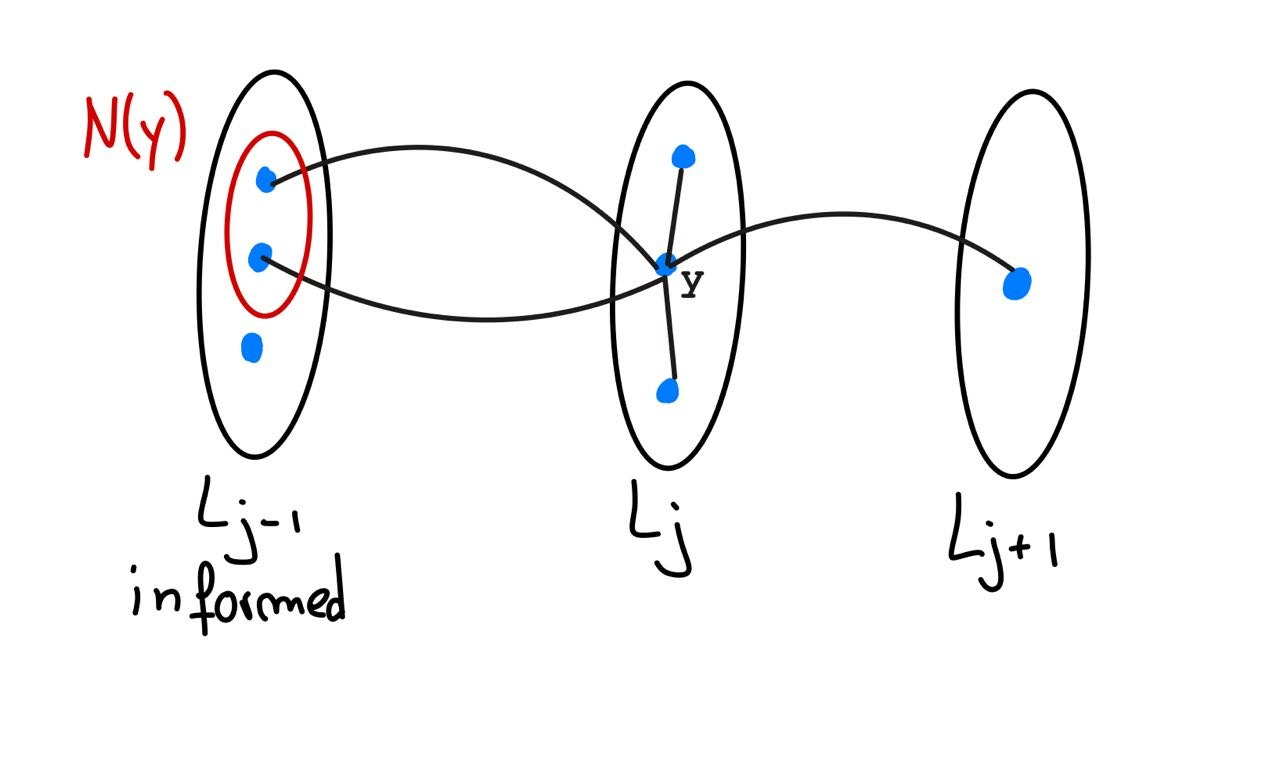
\includegraphics[width=0.6\textwidth]{images/lowerboundRadioNet1.jpg}
                \caption{Per ipotesi induttiva, tutti i nodi a distanza $L_{j-1}$ sono \texttt{informed}.}
            \end{figure}\label{fig:lowerboundRadioNet1}

            Come prima osservazione, notiamo che $N(y) \subseteq V$ e $|N(y)| \leq d$. Poiché $\mathcal{H}$ è una famiglia $(n,d)$-selettiva, per ogni insieme $S \subseteq V$ con $|S| \leq d$ esiste un indice $i \in [t]$ tale che $|S \cap H_i| = 1$. In particolare, questo vale per $S = N(y)$, dunque esiste un time slot $i$ tale che $|N(y) \cap H_i| = 1$.
        \end{description}
    \end{proof}
\end{lemma}

Tuttavia, sorge un problema: la definizione di famiglia selettiva garantisce solo l'esistenza di un $H_i$ tale che esattamente un nodo di $N(y)$ appartiene ad $H_i$, ma non ci dice chi è questo nodo.

\begin{figure}[h]
\centering
\begin{subfigure}[b]{0.48\textwidth}
    \centering
    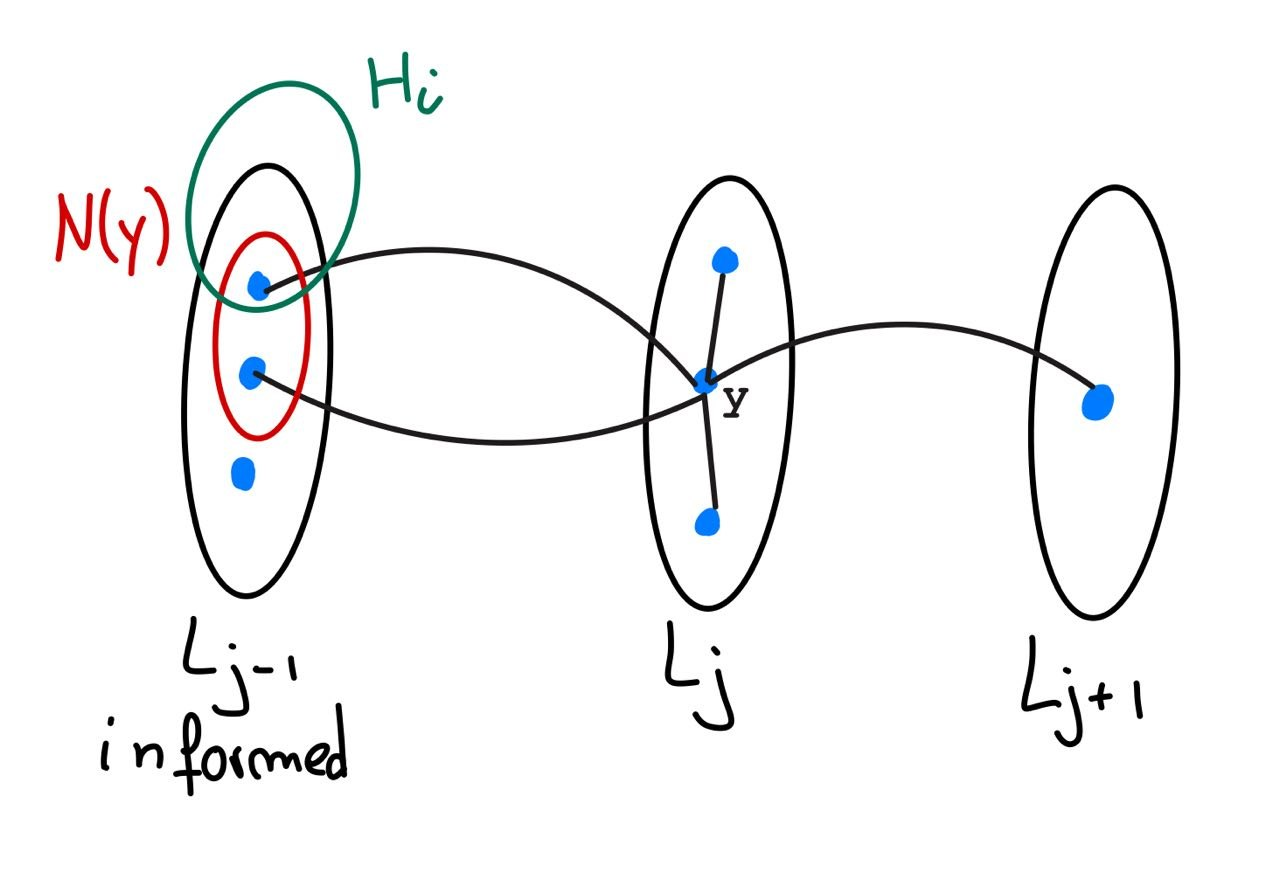
\includegraphics[width=\textwidth]{images/lowerboundRadioNet2.jpg}
    \caption{Caso favorevole.}
    \label{fig:lowerboundRadioNet12}
\end{subfigure}
\hfill
\begin{subfigure}[b]{0.48\textwidth}
    \centering
    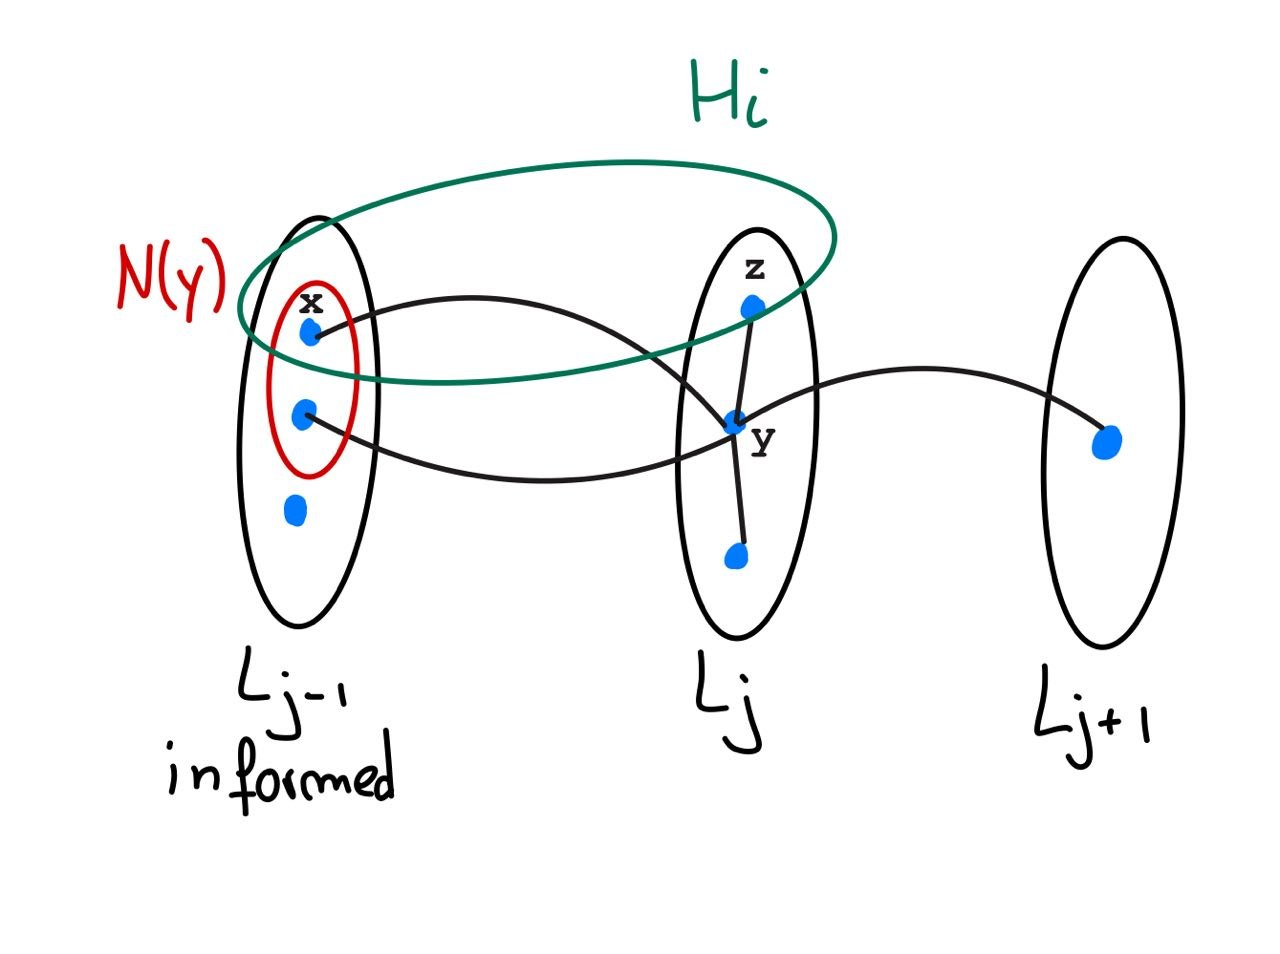
\includegraphics[width=\textwidth]{images/lowerboundRadioNet3.jpg}
    \caption{Caso non favorevole.}
    \label{fig:lowerboundRadioNet3}
\end{subfigure}
\caption{Confronto tra caso favorevole, quando viene scelto un nodo in $N(y)$ informato e caso non favorevole.}
\label{fig:lowerboundRadioNet}
\end{figure}

Il problema risiede nei nodi informati al livello $L_j$ \textbf{durante} la fase $j$. Sia $z \in L_j$ un tale nodo, come illustrato nella \autoref{fig:lowerboundRadioNet3}. Si presentano due casi critici:

\begin{enumerate}
\item Se includiamo $z$ in $N(y)$, la famiglia selettiva potrebbe sceglierlo come unico nodo attivo nell'intersezione $N(y) \cap H_i$, ma poiché $z$ non è ancora informato durante la fase $j$, non trasmetterà alcun messaggio.
\item Se escludiamo $z$ da $N(y)$, esso potrebbe comunque essere già informato e trasmettere simultaneamente ad altri nodi, generando \textbf{collisioni} su $y$.
\end{enumerate}

In entrambi i casi il protocollo fallisce. La soluzione è imporre che durante la fase $j$ siano \textbf{attivi} esclusivamente i nodi che sono stati informati nella fase $j-1$: in questo modo si garantisce che ogni nodo attivo sia effettivamente informato e pronto a trasmettere, eliminando sia il problema della mancata trasmissione sia quello delle collisioni.

Con questa modifica al protocollo, ora il \autoref{lemma:select} è valido, quindi dopo $D$ fasi, tutti i livelli saranno informati. Quindi il tempo di completamento è:
\[
    T = O(D |\mathcal{H}|) = O(D \cdot d \log n)
\]
dove $D = diam(G)$. Dunque, per $D$ e $d$ piccoli, otteniamo un tempo di completamento migliore rispetto al protocollo \texttt{Round-Robin}. Il teorema successivo ci dice inoltre che non possiamo fare di meglio.

\begin{teorema}[Lower Bound]
    Dato un grafo diretto di trasmissione $G=(V,E)$ relativo ad una rete wireless, con diametro $D$, grado massimo $\Delta$ tale che $D\Delta < n$, allora esiste sempre un modo di manipolare i ritardi in modo tale che non si possa risolvere il problema del broadcasting a singola sorgente in un tempo migliore di
    \[
        \Omega(D\Delta \log\left(\frac{n}{D}\right))
    \]
a meno che non si assuma che tutti i nodi conoscano un famiglia $(n,\Delta)$-selettiva di $V$.
\end{teorema}

Per esempio, se consideriamo un grafo con un diametro costante, per esempio $D=3$, avremo che il grado massimo dei nodi $\Delta$ crescerà molto velocemente al crescere di $n$, per esempio in maniera lineare $(\Delta \in O(n))$. Perciò in questo caso avremo un lowerbound di $\Omega(n \log n)$.

Quello che ci si chiede è se esiste un modo per abbattere il fattore $\Delta$ dal lowerbound. Il teorema precedentemente enunciato ci dice che questo è \textbf{deterministicamente} impossibile, perciò è necessario occorrere alla \textit{randomness}.

\section{Probabilistic Protocol}

Definiamo un protocollo probabilistico molto semplice, in cui ogni nodo informato trasmette ai suoi vicini con una certa probabilità $p$ fissata uguale per tutti. È facile mostrare con un controesempio in cui il tempo medio di completamento del protocollo è pessimo.

\begin{figure}[h]
    \centering
    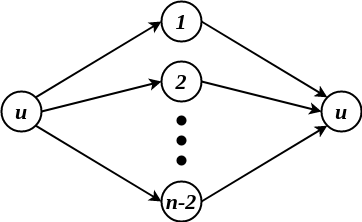
\includegraphics[width=0.4\textwidth]{images/radionet4.png}
    \caption{Controesempio.}
\end{figure}\label{fig:controesempio}

Sia la $u$ la sorgente. Sicuramente esiste un tempo $t_0$ in cui $u$ trasmette il messaggio a tutti i suoi vicini $1, 2, \dots, n-2$ senza interferenze. Dal time slot successivo tutti i suoi vicini inizieranno a trasmettere verso $v$, ognuno con probabilità $p$. Supponiamo per esempio che $p = \frac{1}{2}$, e cerchiamo di stabilire entro quanto tempo ci si aspetta che $v$ verrà informato senza alcuna interferenza. Per prima cosa dobbiamo calcolare con quale probabilità l'evento 
\[
    \mathcal{E} = "v \texttt{ viene informato}"
\]
occorre, e questo si può fare usando la distribuzione binomiale
\[
    P(\mathcal{E}) = \binom{n-2}{1}\frac{1}{2}\left(\frac{1}{2}\right)^{n - 3} = \frac{n-2}{2^{n-2}} \in \Theta\left(\frac{n}{2^n}\right)
\]

Ogni time slot rappresenta un tentativo indipendente in cui l'evento $\mathcal{E}$ ha probabilità $p$ di verificarsi. Aspettare il verificarsi del "primo successo" in una serie di tentativi indipendenti modella esattamente una \textbf{variabile aleatoria geometrica}. Il valore atteso di tale variabile è $1/p$. Si ottiene un tempo di attesa (di completamento del task) $\Theta\left(\frac{2^n}{n}\right)$, che cresce in modo esponenziale.

Anche se $v$ avesse molti meno vicini, per sempio $\sqrt{n}$, il tempo di completamento sarebbe comunque pessimo, $\Theta\left(\frac{2^{\sqrt{n}}}{\sqrt{n}}\right)$

Se inveve $v$ avesse solamente $2$ vicini che trasmettono, il protocollo terminerebbe in tempi brevissimi. Ciò ci suggerisce che dobbiamo trovare un valore di $p$ in modo tale che è \textbf{poco probabile} che avvengano interferenze, ovvero un valore per il quale \textbf{in media} trasmette un solo vicino di ogni nodo. Considerando sempre il precedente controesempio, il valore ottimale per $p$ per il quale i vicini di $v$ devono trasmettere è $\frac{1}{d^{in}(v)}$, ovvero il grado entrante di $v$.

\subsection{BGI Protocol on $d$-Regular Layered Graphs}

Come primo passo consideriamo grafi con strutture che in qualche modo ci semplificano il lavoro. Consideriamo grafi di tipo $d$\textbf{-regular layered}, ovvero grafi suddivisi in \textbf{strati} $L_1, L_2, \dots, L_D$ in cui esistono archi solamente da un livello a quello successivo, e in cui ogn nodo v ha un grado entrante costante a tutti pari a $d^{(in)(v)} = d$. Inoltre esiste una sorgente $s$ tale che $(s,v) \in E \forall v \in L_1$.


\begin{figure}[h]
    \centering
    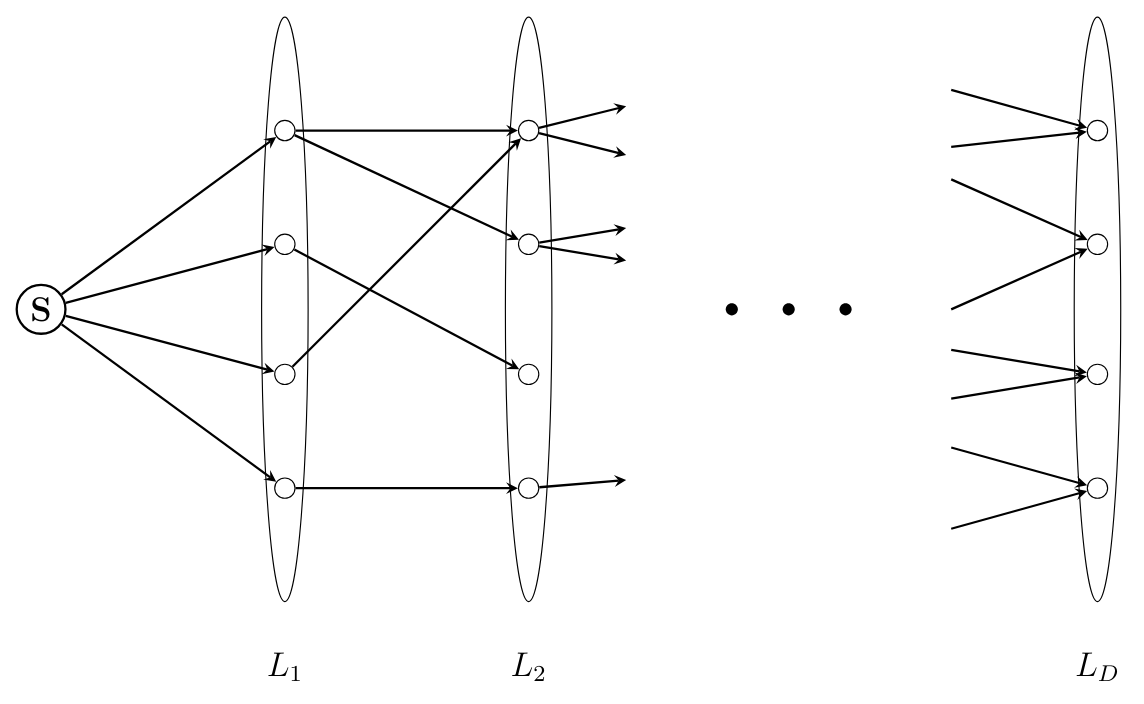
\includegraphics[width=0.4\textwidth]{images/radionet5.png}
    \caption{Esempio di $d$-regular}
\end{figure}\label{fig:dlayered}

Osservare che la descrizione appena data non è propriamente precisa, in quanto i nodi in $L_1$ hanno grado pari ad 1, e quindi non necessariamente $d$, mentre il grado entrante della sorgente $s$ è pari a 0.

\begin{algorithm}
\caption{BGI Protocol}
\begin{algorithmic}[1]
\If{state(x) = \texttt{source}}
    \State \texttt{send(msg)} with probability $p = 1$
\EndIf
\For{stage $k = 1, 2, \dots$}
    \For{time $t =1, 2, \dots, c\log n$}
        \If{$\text{state}(x) = \texttt{informed}$ in stage $k - 1$}
            \State \texttt{send(msg)} with probability $p = \frac{1}{d}$
        \EndIf
    \EndFor
\EndFor
\end{algorithmic}
\end{algorithm}

\begin{teorema}
    Il protocollo \texttt{BGI} su grafi $d$-regular e $D$ layered completa \textit{w.h.p.} il task del broadcast dalla sorgente $s$ in $O(D)$ stages e quindi in $O(D \log n)$ time slots.
    \begin{proof}
        La dimostrazione verrà fatta per induzione sui livelli $j = 1, 2, \dots, D$, ovvero si vuole dimostrare che al termine dello stage $j$ con alta probabilità tutti i nodi del livello $L_j$ saranno informati.

        Il caso per $j = 1$ è banale, perciò assumiamo come \textit{ipotesi iduttiva} che \textbf{con alta probabilità} entro la file dello stage $j > 1$ tutti i nodi nel livello $L_j$ sono già informati (ovvero entro $O(j \log n)$ time slots). Si vuole dimostrare che questo è vero anche per $j + 1$.

        Consideriamo quindi un nodo $v \in L_{j+1}$. Inziamo con calcolare la probabilità che $v$ viene informato in un dato time slot della fase $j+1$. Tale probabilità è pari alla probabilità che uno solo dei suo $d$ \textit{inner-neighbours} trasmette, mentre tutti gli altri $d-1$ non trasmettono, e ciò avviene con probabilità:
        \[
            \binom{d}{1}\frac{1}{d}\left(1 - \frac{1}{d}\right)^{d-1} = \frac{d}{d}\left(1 - \frac{1}{d}\right)^{d-1} = \left(1 - \frac{1}{d}\right)^{d-1}
        \]
        Per valori $d \geq 2$, la quantità $\left(1 - \frac{1}{d}\right)^{d-1} > \frac{1}{8}$ (non ha senso considerare $d = 1$).

        Proseguendo, possiamo dire che il nodo $v$ al livello $j + 1$ non viene informato in un time slot con probabilità al più $1 - \frac{1}{8}$. Quindi

        \begin{align*}
            P(v \text{ non informato in tutti i } c\log n  &\text{ time slot dello stage } j+1) \\
            &< \left(1 - \frac{1}{8}\right)^{c\log n} \\
            &< e^{-\frac{c}{8} \log n} \\
            &= \frac{1}{n^{c/8}}
        \end{align*}
        La prima disuguaglianza è vera perché ogni nodo trasmette in maniera totalmente indipendente dagli altri, mentre la seconda è data dalla seguente espressione
        \[
            1 - x < e^{-x} \quad \forall 0 < x < 1
        \]

        Quindi, se definiamo l'evento
        \[
            \mathcal{E}_v = v \text{ non informato in tutti i } c\log n  \text{ time slot dello stage } j+1
        \]
        occore con al più
        \[
            P(\mathcal{E}_v) \geq \frac{1}{n^{c/8}}
        \]
        Per \textbf{union bound}, possiamo dire che esiste \textbf{almeno un nodo} al livello $L_{j+1}$ che non viene informato entro la fine dello stage $j+1$ occorre con probabilità al più
        \[
            P\left(\cup_{v \in L_{j+1}} \mathcal{E}_v \right) \leq \sum_{v \in L_{j+1}}  P(\mathcal{E}_v) < n \frac{1}{n^{c/8}} = \frac{1}{n^{c/8 - 1}}
        \]
        A questo punto, ponendo $c = 16$, avremo che la probabilità di avere un cosidetto \textit{bad stage} in cui \textbf{non tutti} i nodi del relativo livello vengono informati è al più $\frac{1}{n}$. Possiamo quindi concludere dicendo che ogni nodo $v \in L_{j+1}$ viene informato entro la fine dello stage $j+1$ con probabilità \textbf{almeno} $1 - \frac{1}{n}$, dimostrando così il teorema.
    \end{proof}
\end{teorema}

\subsection{BGI Protocol on General Graphs}
